\chapter{Design and Methodology}
\label{cha:design-and-method}

The goal is to create a web based video player using \ac{DASH} that retrieves the video files through \ac{IPFS}. First, the video quality metrics are explained to give an understanding of how videos are constructed (\autoref{sec:des-video}). This is followed by \autoref{sec:des-dash} which describes how the video files should be split into \ac{DASH} compatible files. Then the intended design used for evaluation is presented in two sections, the first of which is \autoref{sec:des-persona} where user behaviours are presented both in terms of individual users but also collective viewing behaviours. Then in \autoref{sec:des-evaluation} the intended experiments are presented. The viewing experience is meant to be evaluated in many different network conditions with different viewing behaviours.

\section{Frame types and video quality}
\label{sec:des-video}
The images of a video is constructed from a series of pictures called frames. Many video codecs (a program or device used for encoding or decoding audio and/or video) use a \emph{group of pictures} frame structure for compression, which consists of 3 different types of frames (See \autoref{fig:video_compression_frames}).

\begin{itemize}
    \item \ac{I-frame}: An independently coded reference frame, containing the entire picture. This frame type can also be referred to as a keyframe.
    \item \ac{P-frame}: Describes motion changes dependent from last reference frame, containing only the differences from the previous frame.
    \item \ac{B-frame}: Describes motion changes from last and next reference frame, containing only the differences between these frames.
\end{itemize}

\begin{figure}[hb]
    \myfloatalign
    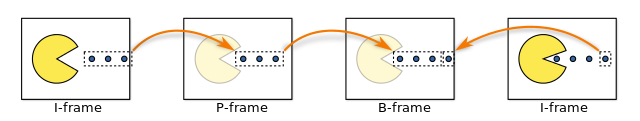
\includegraphics[width=\textwidth]{I_P_and_B_frames}
    \caption[Frame types used in video compression]{A sequence of compressed video frame types, consisting of two keyframes (\acsp{I-frame}), one predicted frame (\acs{P-frame}) and one bi-directionally predicted frame (\acs{B-frame}).}
    \source{\url{https://commons.wikimedia.org/wiki/File:I_P_and_B_frames.svg}}
    \label{fig:video_compression_frames}
\end{figure}

Depending on which type of frame is lost in network traffic, the impact of how many frames are affected varies, i.e. losing an \ac{I-frame} or a \ac{P-frame} causes all frames until next \ac{I-frame} to lose quality, but losing a \ac{B-frame} only affects that single frame as no other frames are dependent on it.

The size also varies: \acp{P-frame} are about half the size of \acp{I-frame}, and \acp{B-frame} are about a quarter the size of \acp{I-frame}\footnote{\url{https://en.wikipedia.org/wiki/Inter_frame}}.

These errors are attempted to be concealed during decoding. The portions of the screen where this is done stay in place until the next \ac{I-frame} or motion changes on that segment of the screen. Videos can also require a re-compression in order to fit into the available bandwidth in which case the image can become blocky or blurry if the compression is too high.
Since \acp{I-frame} contain information on all pixels in the frame, they are always the biggest of the 3 types. Increasing the number of \acp{I-frame} results in fewer prediction errors, but increases the bitrate due to their size.

\section{Preparing video for DASH streaming}
\label{sec:des-dash}
Preparing a video for DASH streaming (also referred to as dashing) involves creating a \ac{MPD} file (See \autoref{sec:rel-dash} and \autoref{fig:mpd_structure}) with meta data such as the used DASH profile specification, the duration of the video, the location of the streams, \etc.

Splitting up videos allows for better \ac{UX}, as less of the video has to be loaded before playback can start. The file segmentation is important to enforce the flow of downloaded files through IPFS, due to a request queue of segments generated by the \ac{DASH} client.

This is possible due to the \ac{DASH} live profile, which supports multiple files (segments) to form a stream. As a consequence of the segmentation each file should begin with an \ac{I-frame}, which could mean that a video needs to be re-encoded to have enough "possible split-points".

Though \ac{DASH} is designed for multiple streams of different bitrates and an adaptive behaviour to maximize the quality of the downloaded content, this aspect will not be examined. Due to the back-end being \ac{P2P}, a single stream of video and audio is chosen to maximize availability of these files. As part of the hypothesis, it is also expected that a single high quality source on \ac{IPFS} can be served equally satisfactorily as several streams in a centralized setup.

\section{Personas}
\label{sec:des-persona}
Possible user behaviours can be used in the experiment, varying between collective and individual behaviours.

Collective behaviours affect the entire network and how the video is watched over time.
\subsection{Collective behaviours}
\begin{itemize}
    \item \textit{Social:}
    Videos accessed through direct link (shared socially) which are candidates for becoming viral. These videos tend to peak in views and then fall off drastically
    \item \textit{Non-social:}
    Videos found through searching or related videos internally on the site. These videos have more stable views over time in comparison to social.
\end{itemize}

\subsection{Individual behaviours}
\label{sec:individual-behavious}
Behaviours can also vary depending on the individual user. The following are possible kinds of users that could use the system.
\begin{itemize}
    \item \textit{Seeder:}
    A user that is sharing content, either being the original poster of said content or re-hosting it after having watched it themselves.

    \item \textit{Binger:}
    A user that watches all content in chronological order.
    
    \item \textit{Leecher:}
    A user that tries to exploit the system, by minimizing the content shared with the other peers.

    \item \textit{Skipper:}
    A user that watches many small segments of the video, by watching a small segment and then skipping forwards to watch another small segment.
    
    \item \textit{Incognito:}
    A user only available in the network for a short time, watching a single video (or part of video) and deletes all of their content afterwards.
    
    \item \textit{Idle:}
    A user that is inside the network but does not actively interact with video content, and as such instead fulfills the role of padding the other clients \acp{DHT}.
\end{itemize}

\subsection{Viewing Conditions}
\label{sec:viewing-conmditions}
Behaviours can also vary depending on the network conditions of the user. The following are different conditions that could influence the usage.
\begin{itemize}
    \item \textit{Normal:}
    Good bandwidth and low latency.
    \item \textit{Mobile:}
    Unreliable due to fluctuating network connections and low bandwidth.
    \item \textit{Remote:}
    High latency due to distance.
\end{itemize}


\section{Evaluation Experiments}
\label{sec:des-evaluation}
Experiments for measuring \ac{QOE}, meaning no re-buffering and stalls of streams:
\begin{itemize}
    \item \textit{Bandwidth:}
    Both the upload and download speeds of the client can be manipulated, and at which point do these become too low to get a pleasant viewing experience, meaning that the video does not halt after it has initially started. Also how does the low upload affect the other peers, and what influence does fluctuating bandwidth capacity have such as that of a mobile client.
    
    Given a video with a static bitrate, $b$, being shared by $s$ seeders in the network, the minimum symmetric bandwidth required for $c$ clients to simultaneously stream the video without stalls is $B$ (See \autoref{eq:bandwidth}).
    
    \begin{equation} \label{eq:bandwidth}
        B = 
        \begin{cases}
            b   &   c \leq s
        \\ \\
            \dfrac{2 \, b \, c - b}{s + c - 1}  &  c > s
        \end{cases}
        \qquad , \qquad 
        c \geq 1 ,
        s \geq 1 
    \end{equation}
    
    This is considered the breaking point of the network, where any speeds below $B$ would result in a bottleneck for sharing of the content and thereby worsen the \ac{UX}.
    
    \autoref{eq:bandwidth} states that if the number of clients wanting the resource is less than or equal to the seeders, the minimum bandwidth required must be the bitrate of the resource. 
    If there are more clients, the needed bandwidth per client must be 2 times the bitrate ($2 \, b \, c$), due to both upload and download, which is then divided among all peers with the resource, except oneself ($s+c-1$).
    Since the data is shared sequentially (starting from a seeder, and then propagating through clients) the last receiving client will not have to share its resource ($-b$). 
    
    \item \textit{Churn rate:}
    What effect does clients leaving the network have on the video. Can videos partially or entirely disappear from the network and can a video be popular enough that this cannot reasonably occur. It makes sense to examine the influence of churn rate on \ac{IPFS}, due to the system's novelty.
   
   \item \textit{Segments availability:}
    How does the socialness and availability of the video impact the user experience and network. The socialness shows the availability over time, while very social videos also have sudden increases in viewership that suddenly drops off. Segments' availability alone can be adjusted by the amount of seeders in the network and can be considered separate from evaluating the impact of different levels of socialness.
    
    \item \textit{Video Quality:}
    Influence of video resolution, \ac{FPS}, time between \acp{I-frame} and bitrate as seen in the testing done by \citeauthor{aloman2015performance}.
    
    \item \textit{Segment size:}
    How does different segment sizes affect the performance. It is expected that if it is too large, one does not properly load balance the requests but if it is too small, enough bytes are not given for the amount of traffic trying to locate the segment.

    \item \textit{Public IPFS:}
    How does \ac{IPFS} perform in a small environment dedicated only to running the tests versus running the test in the public \ac{IPFS} network that is also used for other unrelated services.
    
    \item \textit{Population behaviour:}
    How does the behaviour of the clients in the network affect the network and clients, both themselves and others, with different populations.
\end{itemize}

These tests are to be performed by setting up a \ac{P2P} network containing clients with \ac{IPFS} installed. Each client has a Persona, and tests can be done with different populations of these Personas.

Experiments include:
\begin{itemize}
\item Having different percentages of users being Seeders, as large amount of Seeders increases the availability of the video segments, without other clients having to get them themselves before others can.

\item Different percentages of users being Leechers. A large amount of Leechers is expected to put a high amount of stress on the network as the amount of peers that request files is disproportionally larger than the amount that can supply them.

\item Different percentages of users being idle, this pads the size of the network and can potentially fill up the hash tables of the active peers resulting in slower traffic.

\item Different kinds of user behaviours and how they impact the network compared to each other. This can be tested by having similar networks but the active video watching clients vary between them. The users where this would be relevant for are the Binger, Skipper and the Incognito Personas. Between these users stalling is more tolerable on the Skipper and Incognito Persona as they manually jump to a different points of the video and it is expected upon doing so the video will stall while the buffer is being filled with the relevant segments.
\end{itemize}

\section{Summary of Design and Methodology}
This chapter explained the design of the intended system, where simulated users can view videos through a \ac{DASH} video player. Video compression consists of three different types of frames, \acp{I-frame}, \acp{P-frame} and \acp{B-frame}. These frame types impact the size and quality of a video. The videos can then be split up into segments using the \ac{DASH} standard, so clients can retrieve only the wanted segments, thereby potentially reducing the downloaded data size.

The experiments are intended to be performed with a focus of simulating user behaviours, of which there are two types: Collective and individual. The former describes how viral a video is, and the latter how a user interacts with the video player, characterized in the form of a Persona.

The experiments will evaluate the \ac{UX} gained from the video session by adjusting certain viewing parameters of a user, such as different network conditions, video quality and varying populations of Personas wanting the same video. The experiments are to be done in a simulated \ac{P2P} network.
%%% Local Variables:
%%% mode: latex
%%% TeX-master: "../ClassicThesis"
%%% End:
